\section{Search-Based Reasoning}

\begin{frame}{}
    \LARGE Advanced Reasoning: \textbf{Search-Based Reasoning}

    \vspace{1em}
    \normalsize Given a scorer, is it better to sample many answers or to search step by step?
\end{frame}

\begin{frame}{Three Ways to Use a Verifier}
    \centering
    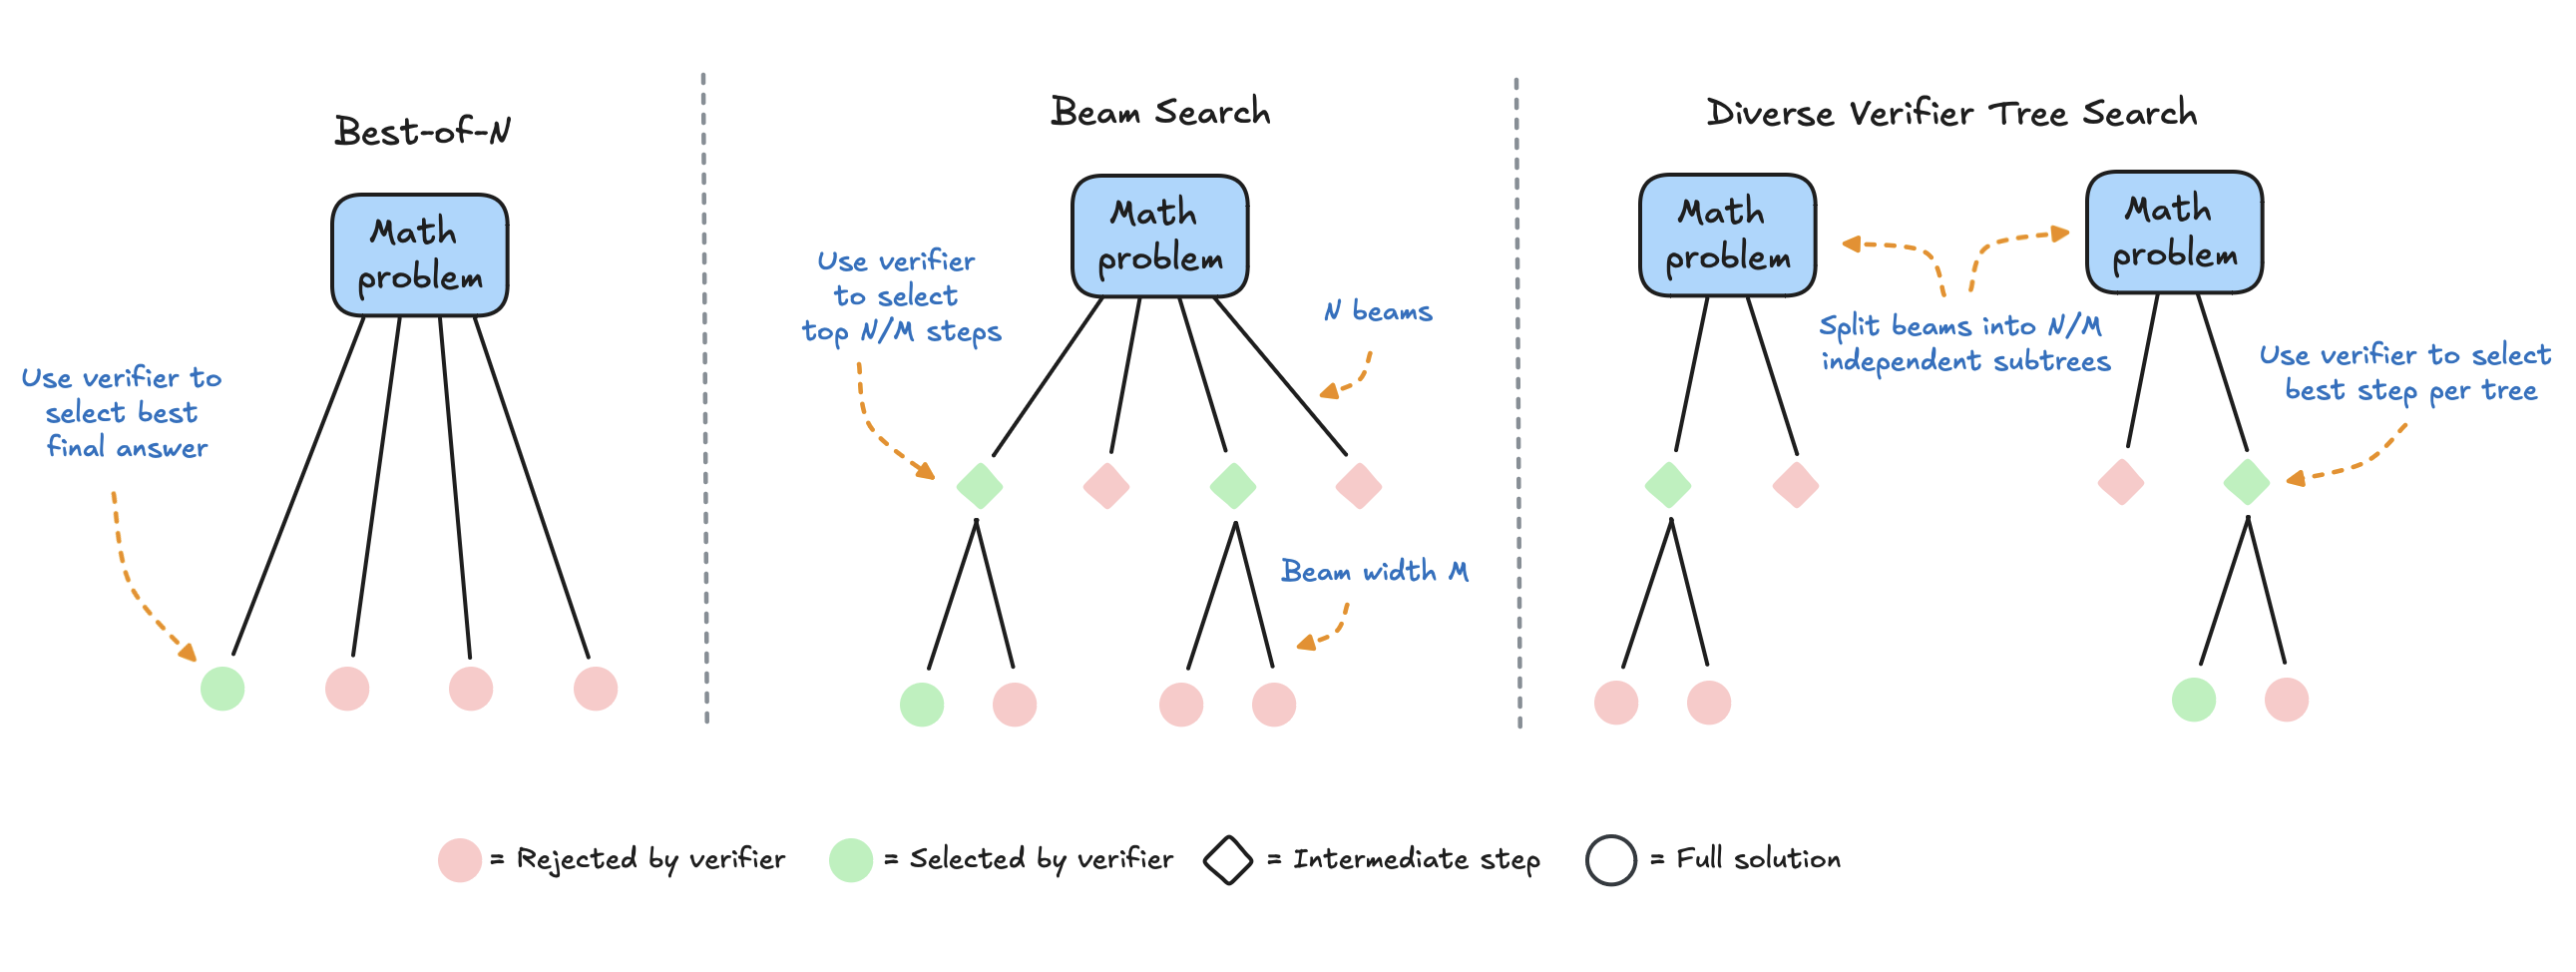
\includegraphics[width=\linewidth,height=0.5\textheight,keepaspectratio]{images/advanced-reasoning/hf_search_strategies.png}
    \begin{itemize}\itemsep0.3em
        \item \textbf{Best-of-N:} score each full solution once, keep the best.
        \item \textbf{Beam search:} score every \emph{step} with a process reward model. Keep the top $N/M$, expand each $M$ ways.
        \item \textbf{DVTS:} split the budget into $N/M$ independent subtrees. Less exploitation, more diversity.
    \end{itemize}
    \src{Figure: Beeching, Tunstall and Rush (Hugging Face), ``Scaling test-time compute with open models'' (2024). Beam search with a process reward model follows Snell et al., \href{https://arxiv.org/abs/2408.03314}{arXiv:2408.03314}.}
\end{frame}

\begin{frame}{Aggregation, and Why It Saturates}
    \begin{itemize}\itemsep0.05em
        \item With samples $y^{(1)},\dots,y^{(N)}$, answers $a_i$ and a scorer $v$:
        \[
            \underbrace{\arg\max_{y^{(i)}} v\big(y^{(i)}\big)}_{\text{best-of-N}}
            \qquad
            \underbrace{\arg\max_a \sum_{i} \mathbb{1}[a_i=a]}_{\text{majority vote}}
            \qquad
            \underbrace{\arg\max_a \sum_{i} v\big(y^{(i)}\big)\,\mathbb{1}[a_i=a]}_{\text{weighted vote}}
        \]
        \item \textbf{A limit theorem.} As $N\to\infty$, voting accuracy converges to a value fixed by the generator $g$ and the scorer $v$. To pass it, improve $v$ or $g$.
        \item \textbf{Best-of-N is optimisation against a proxy.} With $d=\sqrt{D_{\mathrm{KL}}(\pi\,\|\,\pi_{\text{init}})}$ and $\mathrm{KL}_{\text{bon}}=\log n-\tfrac{n-1}{n}$, the \emph{true} reward follows
        \[
            R_{\text{bon}}(d)=d\,(\alpha_{\text{bon}}-\beta_{\text{bon}}\,d)
        \]
        It rises, peaks, then \alert{falls}: with a large enough $N$ you select what fools the scorer.
        \item \textbf{A ceiling from false positives.} Resampling cannot lower a verifier's false-positive rate. The optimal number of attempts is then rarely above 10.
    \end{itemize}
    \vspace{0.1em}
    \src{Welleck, CMU 11-711 (Nov 2025). Wu et al., \href{https://arxiv.org/abs/2408.00724}{arXiv:2408.00724}, Theorem 2. Gao, Schulman and Hilton, ``Scaling Laws for Reward Model Overoptimization,'' \href{https://arxiv.org/abs/2210.10760}{arXiv:2210.10760}. Stroebl, Kapoor and Narayanan, \href{https://arxiv.org/abs/2411.17501}{arXiv:2411.17501} (abstract).}
\end{frame}

\begin{frame}{Search Is Not Uniformly Better than Sampling}
    \begin{columns}[T,onlytextwidth]
        \column{0.46\textwidth}
        \centering
        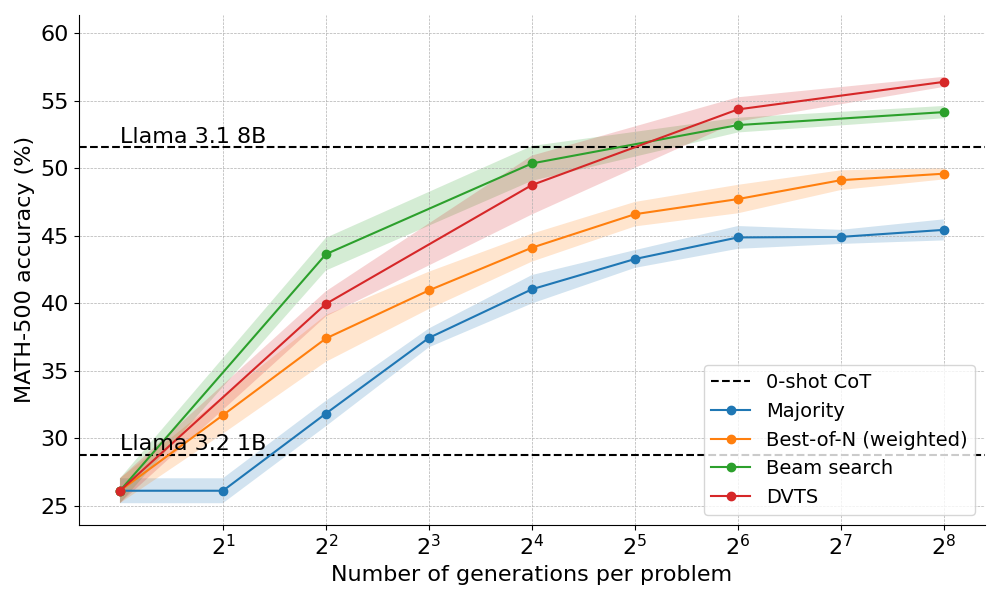
\includegraphics[width=\linewidth,height=0.58\textheight,keepaspectratio]{images/advanced-reasoning/hf_methods_all.png}

        {\scriptsize Llama 3.2 1B on MATH-500, with an 8B process reward model}
        \column{0.52\textwidth}
        \begin{itemize}\itemsep0.4em
            \item \textbf{At small budgets, beam search wins.} Beam with 4 generations matches best-of-N with 16. Beam with 16 matches best-of-N with 256.
            \item \textbf{At large budgets on easy problems, it loses.} The beam over-exploits the reward model. DVTS restores diversity.
            \item \textbf{REBASE} spreads the budget by score, $W_j\propto e^{R(n_j)/T_b}$, with no rollouts. About 7$\times$ less compute than sampling.
            \item A 3B model with the right strategy per difficulty passes Llama 3.1 70B, with about 22$\times$ fewer parameters.
        \end{itemize}
    \end{columns}
    \vspace{0.1em}
    \src{Beeching, Tunstall and Rush (Hugging Face), ``Scaling test-time compute with open models'' (2024). Snell et al., \href{https://arxiv.org/abs/2408.03314}{arXiv:2408.03314}. Wu et al., \href{https://arxiv.org/abs/2408.00724}{arXiv:2408.00724}.}
\end{frame}

\begin{frame}{Monte Carlo Tree Search on Text}
    \begin{columns}[T,onlytextwidth]
        \column{0.5\textwidth}
        \centering
        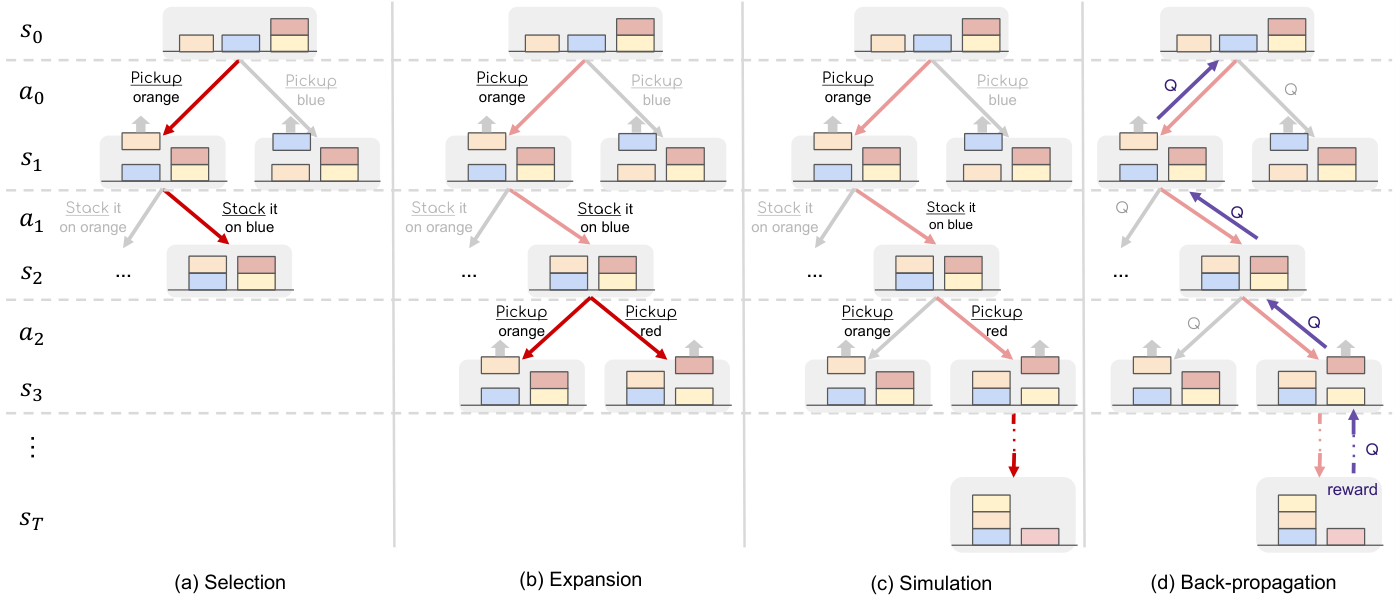
\includegraphics[width=\linewidth,height=0.4\textheight,keepaspectratio]{images/advanced-reasoning/rap_mcts_phases.png}

        \vspace{0.2em}
        \small
        \begin{adjustbox}{max width=\linewidth}\begin{tabular}{lccc}
            \toprule
            \textbf{Blocksworld steps} & \textbf{2} & \textbf{4} & \textbf{6} \\
            \midrule
            CoT, LLaMA-33B & 0.17 & 0.02 & 0.00 \\
            CoT, GPT-4 & 0.50 & 0.63 & 0.40 \\
            \rowcolor{KAUSTcyan!12} RAP, 20 iterations & 1.00 & 0.88 & 0.42 \\
            \bottomrule
        \end{tabular}\end{adjustbox}
        \column{0.48\textwidth}
        \begin{itemize}\itemsep0.4em
            \item \textbf{The mapping.} A node is a partial reasoning trace. An action is the next step. The value comes from rollouts, self-evaluation or a learned model.
            \item \textbf{Selection} balances value against novelty:
            \[
                a^*=\arg\max_{a}\Big[Q(s,a)+w\sqrt{\tfrac{\ln N(s)}{N(c(s,a))}}\Big]
            \]
            \item \textbf{RAP:} the LLM plays two roles. It proposes actions, and it is the \emph{world model} that predicts the next state.
            \item A small model with search beats GPT-4 with CoT: 64\% average.
        \end{itemize}
    \end{columns}
    \vspace{0.1em}
    \src{Hao et al., ``Reasoning with Language Model is Planning with World Model,'' EMNLP 2023, \href{https://arxiv.org/abs/2305.14992}{arXiv:2305.14992}, Eq. 1 and Table 1. Rush and Ritter, ``Speculations on Test-Time Scaling'' (2024).}
\end{frame}

\begin{frame}{rStar-Math: Search as a Data Generator}
    \centering
    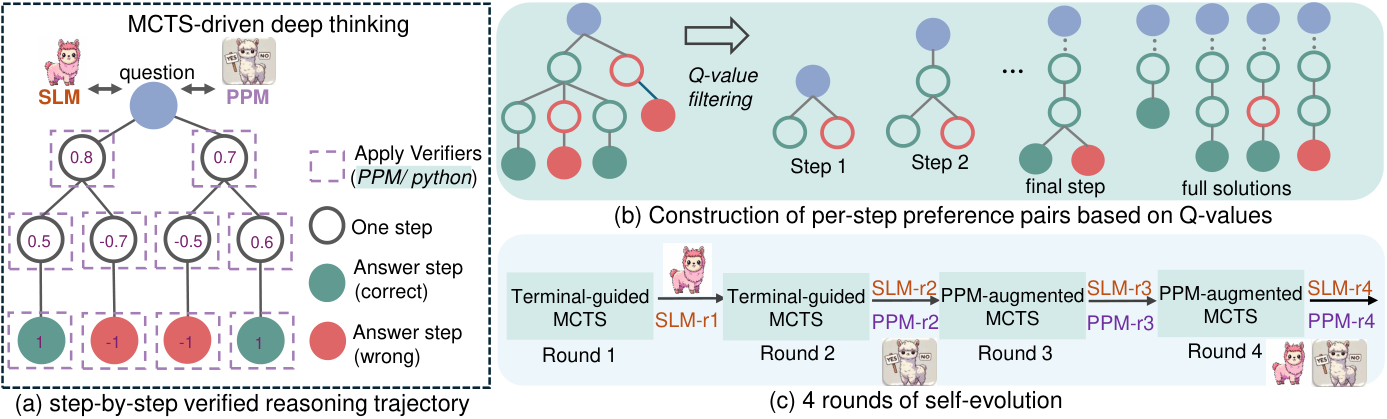
\includegraphics[width=\linewidth,height=0.4\textheight,keepaspectratio]{images/advanced-reasoning/rstar_math_method.png}
    \begin{itemize}\itemsep0.25em
        \item \textbf{Each node is text plus Python.} A step whose code fails is dropped. Four rounds of self-evolution improve policy and scorer together.
        \item \textbf{A preference model, not a value regressor.} Q-values from rollouts are noisy, so train on pairs:
        $\mathcal L_{\text{ppm}}=-\tfrac14\,\mathbb E\big[\log\sigma\big(r_\theta(x,y^{\text{pos}})-r_\theta(x,y^{\text{neg}})\big)\big]$.
        \item Qwen2.5-Math-7B on MATH: 58.8\% to \textbf{90.0\%}. AIME 2024: 8 of 15. The model also learned to abandon a flawed approach and backtrack, without being trained to.
    \end{itemize}
    \src{Guan et al. (Microsoft Research Asia), ``rStar-Math: Small LLMs Can Master Math Reasoning with Self-Evolved Deep Thinking,'' \href{https://arxiv.org/abs/2501.04519}{arXiv:2501.04519}.}
\end{frame}

\begin{frame}{Why Frontier Labs Skipped Tree Search}
    \begin{itemize}\itemsep0.3em
        \item In late 2024, AlphaZero-style search was a leading guess about how o1 was built. Then came the open recipes.
        \item \textbf{DeepSeek-R1, ``Unsuccessful Attempts'':}
        \begin{itemize}\itemsep0.15em
            \item token generation has an exponentially larger search space than chess or Go
            \item capping the expansions per node traps the search in local optima
        \end{itemize}
        \item \textbf{Kimi k1.5:} planning can be \emph{approximated inside the context}. Thought tokens play the role of a planning budget.
        \item \textbf{The verdict in the lecture halls:} R1 ``ended speculations on the necessity of MCTS''. Later models for hard maths do add structure, though not classical MCTS.
    \end{itemize}
    \vspace{0.1em}
    \takeaway{\textbf{Where explicit search survives:} where a terminal check is cheap and exact (code, formal maths), and as a \emph{generator of training data}.}
    \src{DeepSeek-AI, \href{https://arxiv.org/abs/2501.12948}{arXiv:2501.12948}, Appendix G.2 (v2). Kimi Team, \href{https://arxiv.org/abs/2501.12599}{arXiv:2501.12599}, Sections 2.3 and 4. Hashimoto, Stanford CS336 Lecture 16 (2025). Choi, Stanford CS224N Lecture 12 (2026). Rush and Ritter (2024).}
\end{frame}

\begin{frame}{Better Selectors for Parallel Samples (2025)}
    \centering
    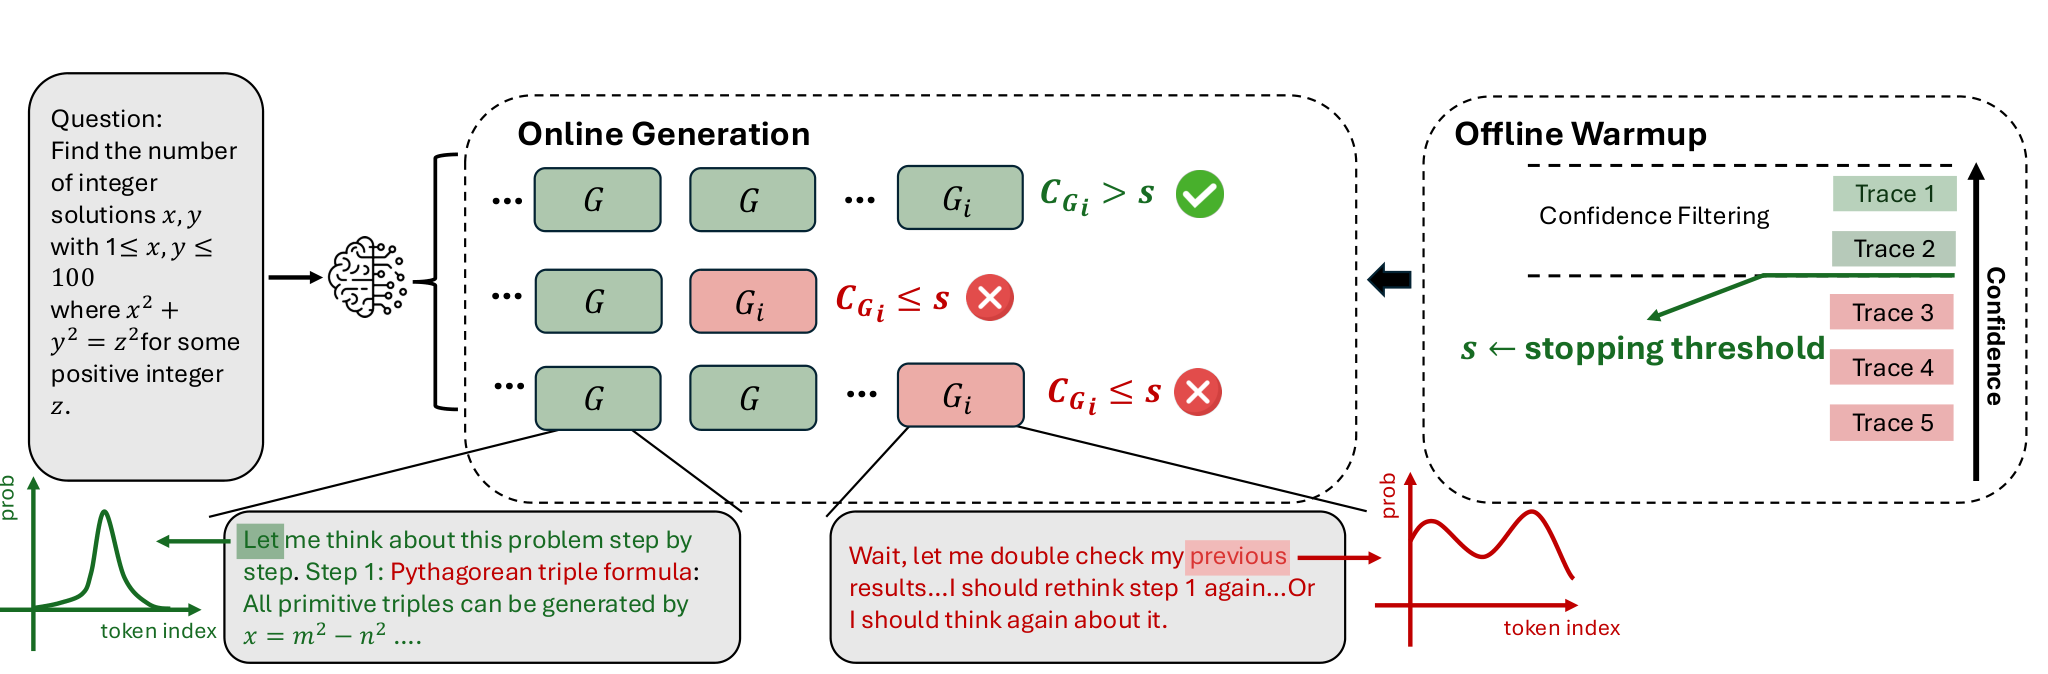
\includegraphics[width=\linewidth,height=0.42\textheight,keepaspectratio]{images/advanced-reasoning/deepconf_online.png}
    \begin{itemize}\itemsep0.3em
        \item \textbf{DeepConf: use the model's own confidence.} Score a trace by its \emph{weakest} window. Warm up on 16 traces, then \textbf{stop any trace that drops below the threshold}.
        \item gpt-oss-120b, AIME 2025, budget 512: majority vote 97.1\%. DeepConf 97.9\% with \textbf{84.7\% fewer tokens}.
        \item \textbf{GenSelect: let a reasoning model choose} among all candidates in one prompt. QwQ-32B, 64 candidates: majority 68.4\%, GenSelect \textbf{73.4\%}.
    \end{itemize}
    \src{Fu et al. (Meta AI, UCSD), ``Deep Think with Confidence,'' \href{https://arxiv.org/abs/2508.15260}{arXiv:2508.15260}. Toshniwal et al. (NVIDIA), ``GenSelect,'' \href{https://arxiv.org/abs/2507.17797}{arXiv:2507.17797}.}
\end{frame}

\begin{frame}{Search: What to Remember}
    \begin{itemize}\itemsep0.6em
        \item Best-of-N, beam search and MCTS differ in \textbf{where the scorer is applied}: once per answer, or once per step.
        \item Step-level search wins at \textbf{small budgets and on hard problems}. It loses when it over-exploits the scorer.
        \item Voting and re-ranking \textbf{saturate}. The limit is set by the generator and the scorer, not by $N$.
        \item Explicit tree search did not become the route to reasoning models. It became a \textbf{data generator}, and a tool where checks are exact.
    \end{itemize}
    \vspace{0.3em}
    \vspace{0.3em}
    \takeaway{\textbf{Next.} Every method here leaned on a scorer of steps or of answers. How are such scorers built, and can they be trusted?}
\end{frame}
